\subsection{Arquitectura del sistema}

	En el flujo de trabajo de la presente tesis, ilustrado en la Figura \ref{fig:workflow}, se destacan dos herramientas interconectadas como parte central de la solución propuesta: el RNA y el ACG. Como se ilustra en la Figura \ref{fig:architecture}, existen diferentes módulos a considerar en cada una de las dos herramientas. Los módulos en amarillo corresponden a las clases implementadas en base al estándar railML, los módulos en verde son aquellos algoritmos originales necesarios para resolver el problema, y finalmente los módulos en violeta constituyen todas las validaciones realizadas.

    \begin{figure}[H]
        \centering
        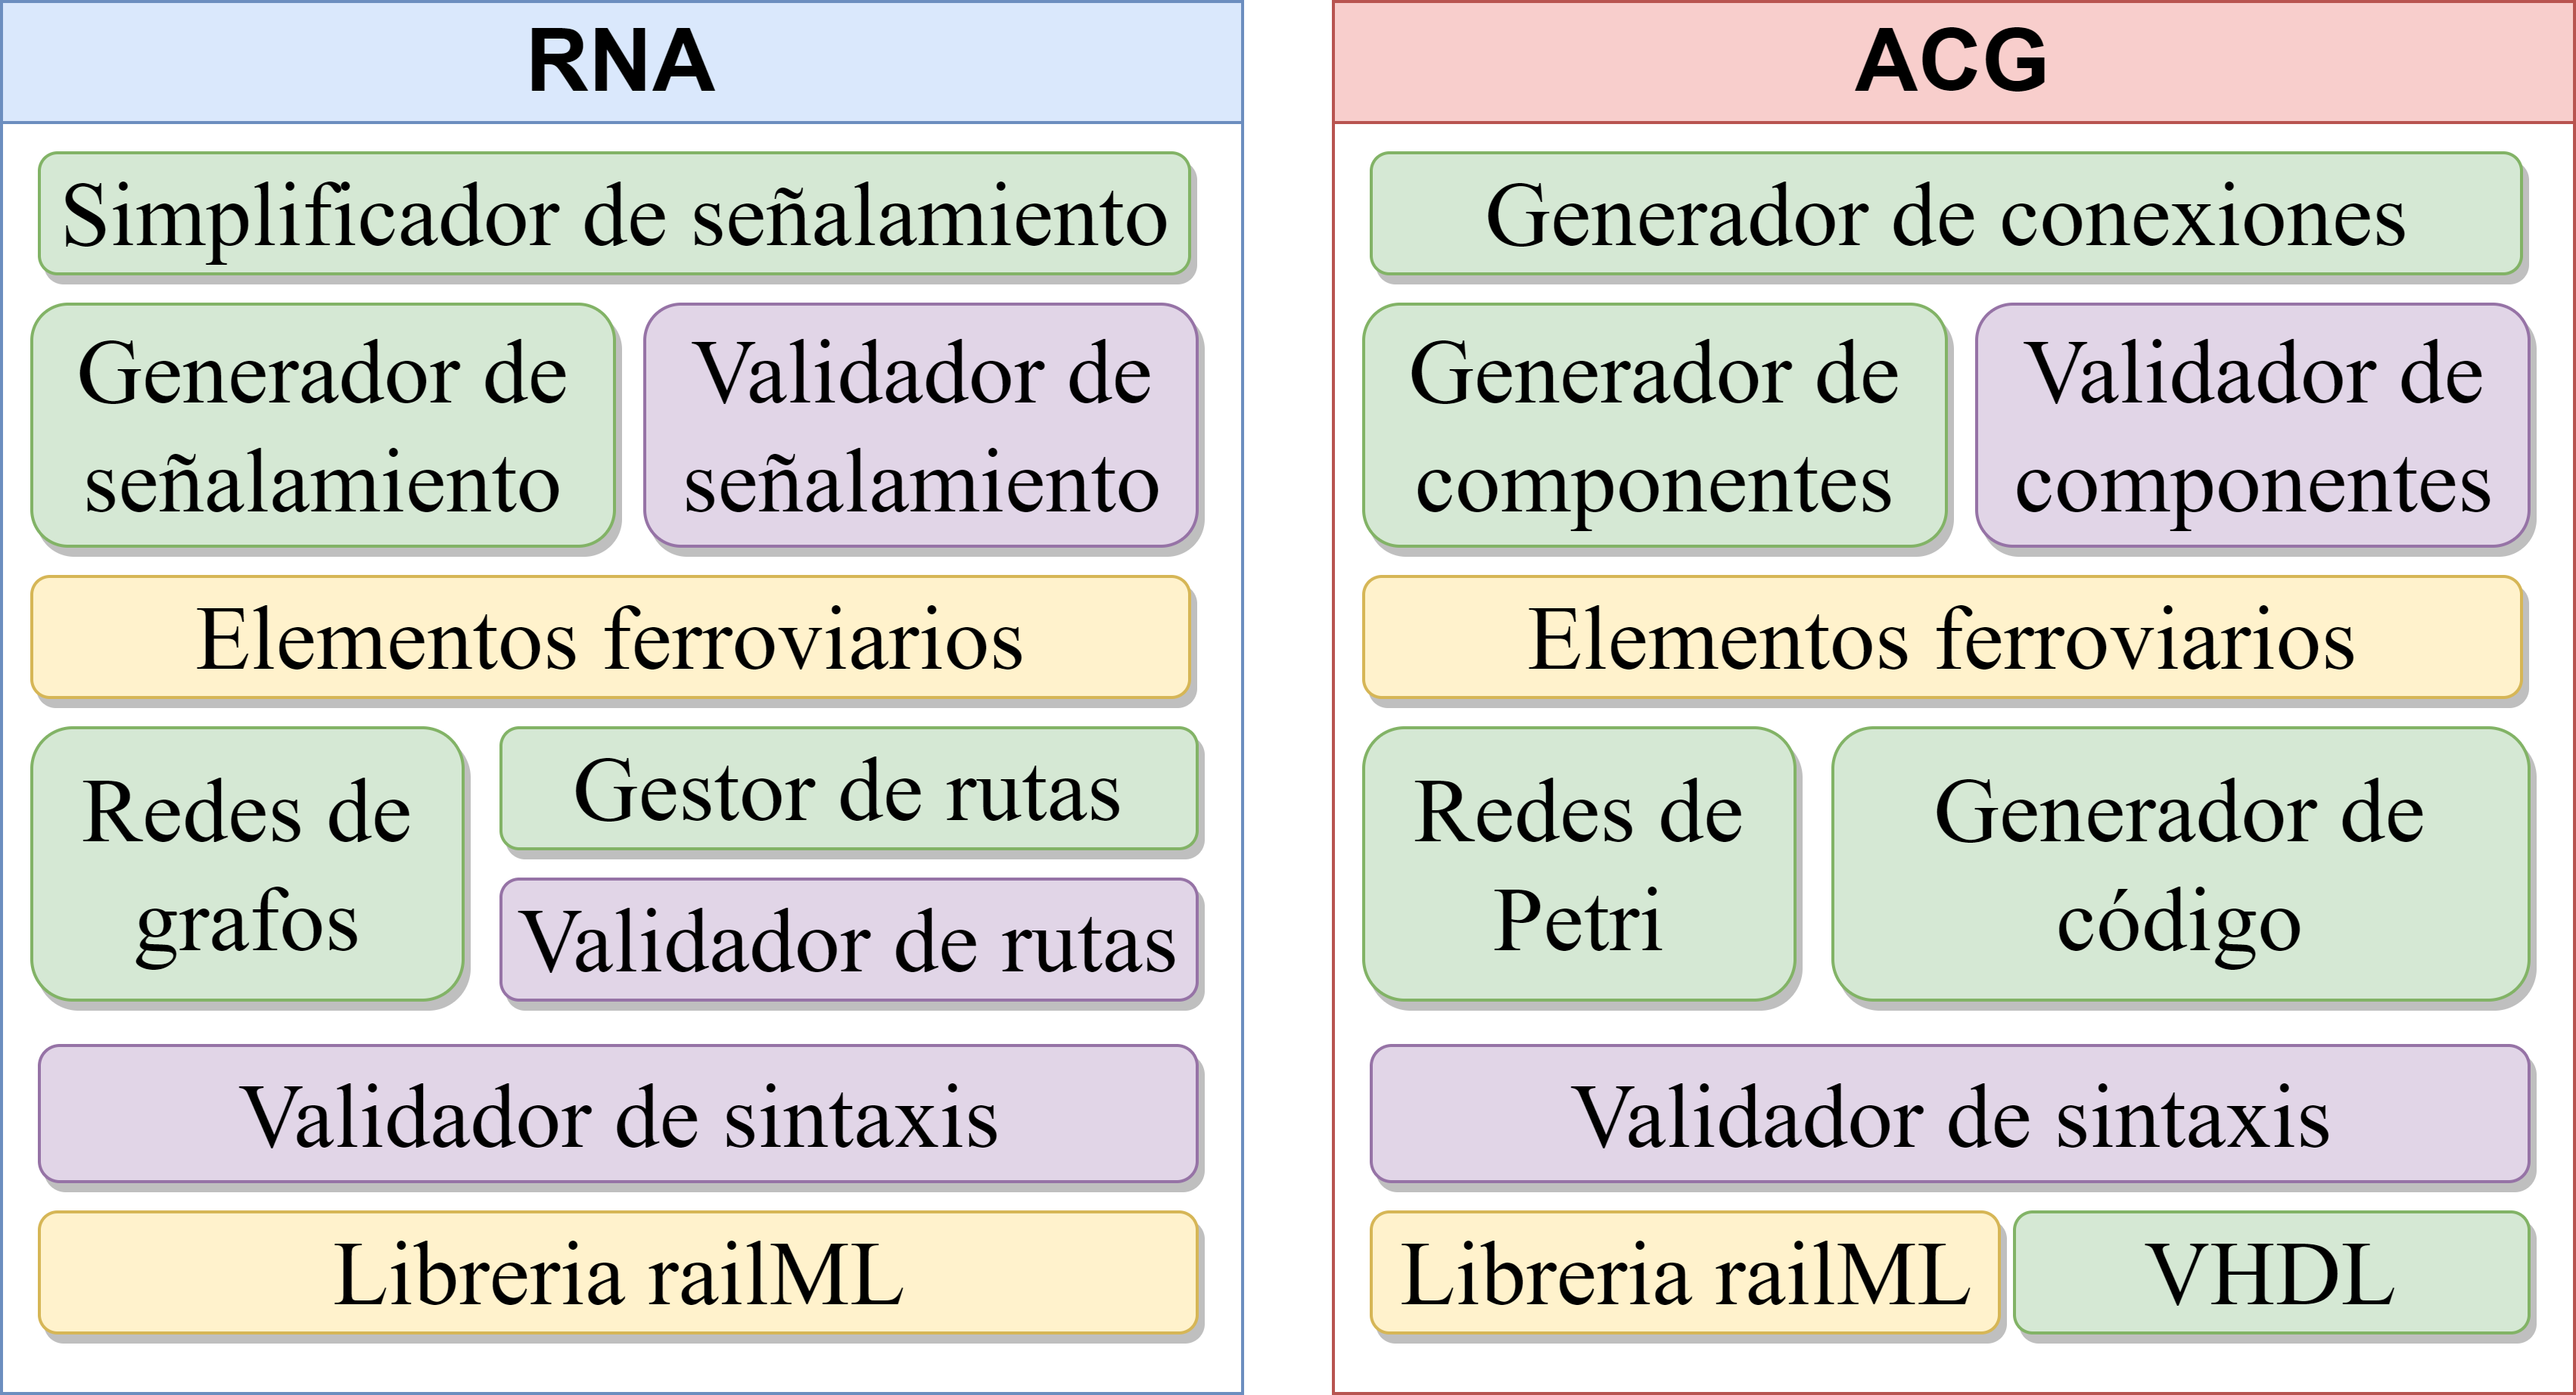
\includegraphics[width=1\textwidth]{Figuras/Architecture.png}
        \centering\caption{Arquitectura del sistema}
        \label{fig:architecture}
    \end{figure}

    Las clases implementadas se corresponden una a una con las definidas en el estándar railML. De esta manera, cualquier elemento definido en un archivo railML tendrá su equivalente en el modelo de datos utilizado. La biblioteca a implementar debe ser capaz de importar, modificar y exportar archivos en formato railML. Además, la librería debe contemplar todos los atributos que railML defina para cada elemento ferroviario.

    Respecto al RNA, el análisis de redes de grafos es explicado en la Sección \ref{sec:grafos}, la generación de señalamiento en la Sección \ref{sec:generacion}, la simplificación del señalamiento en la Sección \ref{sec:simplificacion} y, finalmente, la generación de rutas ferroviarias y la tabla de enclavamientos es explicado en la Sección \ref{sec:rutas}. En tanto que para el ACG, la descripción de cada bloque implementado se encuentra explicada en la Sección \ref{sec:interlockingArch}, la implementación de la redundancia en la Sección \ref{sec:VHDL2oo3} y la plataforma utilizada se explica en la Sección \ref{sec:AGG}.